%1_introduction.tex
%notes for the course Algorithms COMS10007 taught at the University of Bristol
%2017_18 Conor Houghton conor.houghton@bristol.ac.uk

%To the extent possible under law, the author has dedicated all copyright 
%and related and neighboring rights to these notes to the public domain 
%worldwide. These notes are distributed without any warranty. 

\documentclass[11pt,a4paper]{scrartcl}
\typearea{12}
\usepackage{graphicx}
%\usepackage{pstricks}
\usepackage{listings}
\usepackage{color}
\lstset{language=C}
\pagestyle{headings}
\markright{COMS10007 1\_introduction (a/b, start of c) - Conor}
\begin{document}

\section*{1: Introduction}

\subsection*{Algorithms}

This course is about algorithms and data structures; roughly speaking,
an algorithm is a clearly defined list of manipulations which can be
applied to data to achieve an objective and a data structure is a way
to store information. The word algorithm comes from the name of the
great ninth century Persian astronomer and mathematician
al-Khw\-{a}rizm\-{i}. 

We've always had algorithms, counting beads for tallying, the
Babylonian algorithm for solving quadratic equations, the Chinese
remainder theorem for solving congruence equations; for much of
history the idea of an algorithm has been a part of applied
mathematics, a method for working something out. Now, with computers
the study of algorithms has become a seperate discipline, with
abstract questions about computibility and practical ones about how to
evaluate algorithms and chose between available algorithms for a
particular application.

Algorithms are the part of a programme that don't generally depend
on the hardware or programming language. This isn't to say that some
programming lanaguages don't express some algorithms for naturally or
more easily and that some compilers aren't better or worse at
optimizing certain algorithms and there is lots of variability, for
example, in how well recursion runs from language to language,
compiler to compiler and chip to chip. However, the aim in examining
algorithms is to do so in a platform independent way. This isn't to
say we won't use a platform, examples will be given in C and you will
be encouraged to try out the algorithms using your knowledge of C and
Haskell programming.

\subsection*{Sorting - Insertion Sort}

Discussions of algorithms tend to involve lots of discussions of
sorting. This is partly because sorting is a big issue, search and
sort algorithms are important in the analysis of data, be it
scientific data or web addresses and data analysis is at the heart of
contemporary technological revolution. The other part is that sorting
is a particularly good illustrative example.

Consider sorting a pack of card, using bridge ordering, clubs,
diamonds, hearts, spades, the goal is to order the cards so the ace of
clubs is at the bottom and the king of spades at the other. To make it
more straight forward, imagine they are numbered one, for the ace of
clubs, through to 52 for the king of spades, that makes it less
confusing to talk about one card having a value less than another.

The obvious way to sort is probably the algorithm known as
\emph{insertion sort}.  Take the unsorted deck, the cards will be
added one by one to another deck, the sorted deck, with, for the sake
of definiteness, the lowest card at the bottom, the highest on top and
all the others in order in between. First, take the first card in the
pack and put it in the other deck, the sorted deck now has exactly one
card in it. Now take the second card in the unsorted deck and put it
above or below the first according to whether it has a higher or lower
value. After that, keep going, take a card from the unsorted deck,
search through the sorted deck from the top until the next card has a
smaller value than it and put it in above that card. When all the
cards are gone from the unsorted deck, the algorithm is complete. An
example of insertion sort is given in Table~\ref{tab_insertsort}.

\begin{table}
\begin{tabular}{r|cccccc}
1&&4&2&0&1&3\\
2&4&&2&0&1&3\\
3&4&2&&0&1&3\\
4&2&4&&0&1&3\\
5&2&4&0&&1&3\\
6&2&0&4&&1&3\\
7&0&2&4&&1&3\\
8&0&2&4&1&&3\\
9&0&2&1&4&&3\\
10&0&1&2&4&&3\\
11&0&1&2&4&3&\\
12&0&1&2&3&4&
\end{tabular}
\caption{An insertion sort example. A space divides the sorted deck
  from the unsorted deck; in practice this isn't needed, the sorted
  and unsorted elements can be stored in the same array with an index
  or pointer used to remember where one stops and the other
  starts. Consider, for example, steps \textbf{ 7} to \textbf{ 10} where the
  value 1 is moved to the sorted deck and then compared with each of
  the sorted values until it reaches the 0, since the 0 is a lower
  value than 1 the 1 isn't swapped with it and the algorithm goes on
  to move the 3 into the sorted deck.\label{tab_insertsort}}
\end{table}

\subsubsection*{Implementation and run speed}

A C function for sorting is given in Table~\ref{c_insertsort}; this is
a function, to see it in action download \texttt{insert\_sort.c}. Now,
the question is, how good an algorithm is this. Of course, \lq{}how
good\rq{} could mean lots of different things, depending on what
constraints there are on the use of the program, it could mean the
size of the program itself, or the amount of memory the program needs
for data storage, but most frequently, it means run time.


\begin{table}
\begin{lstlisting}[numbers=left]
void sort(int a[],int n)
{

   int i,j,this_a;

   for(i=1;i<n;i++){
      this_a=a[i];
      j=i-1;

      while(j>=0&&this_a<a[j]){
         a[j+1]=a[j];
	 j=j-1;
      }

      a[j+1]=this_a;
   }
}
\end{lstlisting}
\caption{A function for sorting an array. This function can be found
  included in the program \texttt{insert\_sort.c}. It takes as an
  argument an array of ints called \texttt{a[]} and \texttt{n}, the
  size of the array and sorts it using insert sort. The array is
  sorted from \texttt{a[0]} and the sorted elements are stored in the
  same array, with i marking at each iteration the last element in the
  sorted deck, the while loop moves the element that was \texttt{a[i]}
  into the correct place.\label{c_insertsort}}
\end{table}

Lets examine the run time for the function in
Table~\ref{c_insertsort}. Let $n$ be the number of elements in the
list. The amount of time each line takes to run is platform dependent,
so lets say the run time for the $i$th line is $t_i$:
\begin{equation}
t_i=\mbox{time it takes line }i\mbox{ to run once}
\end{equation}
Lets call the total run time $T(n)$ since it depends on $n$, the
number of elements that need sorting and the contribution to $T(n)$ of
the $i$th line $T_i$, 
\begin{equation}
T_i=\mbox{the total time the program spends on line }i
\end{equation}
Now $T_i\not= t_i$ in general because some lines run more than once,
here, for example, $T_4=t_4$ since the fourth line only runs once, but
$T_7=(n-1)t_7$, once for each value of $i$. $T_6$ is a bit more
complicated in an uninteresting way since the end condition $i<n$ is
checked $n$ times, the initial condition $i=1$ only happens once and
the increment happens $n-2$ times, but lets approximate and say
$T_6=nt_6$.

Lines \textbf{11} and \textbf{12} are complicated in a more
interesting way, we don't know how many times \texttt{j} needs to be
reduced until the while condition returns false, it depends on the
value of \texttt{a[i]} and the values of the elements already
sorted. Obviously, if the list is already sorted then the while
condition fails each time and these lines are never run; this is an
exceptional case however. Conversely, in the worst case the sequence
starts of in reverse order, in which case lines \textbf{11} and
\textbf{12} run $i$ times for each value of $i=1$ to $i=n-1$, thus
\begin{equation}
T_{11}=\sum_{i=1}^{n-1}i t_{11}=\frac{1}{2}n(n-1) t_{11}
\end{equation}
The formula used to calculate this is explained in
Table~\ref{math_sum_of_digits}. Line \textbf{10} is a bit like line
\textbf{6}, it is run one extra time so
\begin{equation}
T_{10}=\sum_{i=1}^{n-1}(i+1) t_{10}=\frac{1}{2}(n+1)n t_{10}
\end{equation}
All these precise sums are being calculated this time for illustrative
reasons, in fact, the point we will make is that the only thing that
is really of interest is the power of the highest power of $n$ and
detailed calculations like this won't be done again.

\begin{table}
So there is formula for summing all the numbers from one to $n$:
\begin{equation}
\sum_{i=1}^ni = \frac{n(n+1)}{2}
\end{equation}
This can be proved by induction. If $n=1$ it holds with one on each
side of the equation. Now assume it holds for $n-1$ and consider
\begin{equation}
\sum_{i=1}^ni=n+\sum_{i=1}^{n-1}i=n+\frac{1}{2}n(n-1)=\frac{n(n+1)}{2}
\end{equation}
proving the formula by induction.
\caption{Mathematical aside: the formula for adding numbers. \label{math_sum_of_digits}}
\color{black}
\end{table}

Now we can calculate $T(n)$ for the worst case.
\begin{eqnarray}
T(n)&=&t_1+t_4+nt_6+(n-1)(t_7+t_8+t_{15})\cr&&+\frac{1}{2}(n+1)nt_{10}+\frac{1}{2}n(n-1)(t_{11}+t_{12})
\end{eqnarray}
Gathering everything together this has the form
\begin{equation}
T(n)=an^2+bn+c
\end{equation}
where, for example $a=(t_{10}+t_{11}+t_{12})/2$. What we see is that
the coefficients, $a$, $b$ and $c$ are complicated, they depend on the
run times of individual lines of code, the balance between the $n^2$
and $n$ terms is similarly hard to evaluate. In short, the most
interesting and definite platform independent statement we can make
about $T(n)$ is that it grows like $n^2$ as $n$ becomes large. We say
\begin{equation}
T(n)\in O(n^2)
\end{equation}
The $n^2$, the fastest growing term in the expression for $T_n$ is
sometimes called the leading term. This will be discussed further, but
first have a look at Fig.~\ref{fig_insert_sort_timing} where the run
time of the program is plotted against $n$ for $n\in(1,1000)$. We see
that the curve is extremely well matched by $n^2$, the sub-leading
order terms, the $n$ term and the constant, aren't important.

\begin{figure}
% GNUPLOT: LaTeX picture with Postscript
\begingroup
  \makeatletter
  \providecommand\color[2][]{%
    \GenericError{(gnuplot) \space\space\space\@spaces}{%
      Package color not loaded in conjunction with
      terminal option `colourtext'%
    }{See the gnuplot documentation for explanation.%
    }{Either use 'blacktext' in gnuplot or load the package
      color.sty in LaTeX.}%
    \renewcommand\color[2][]{}%
  }%
  \providecommand\includegraphics[2][]{%
    \GenericError{(gnuplot) \space\space\space\@spaces}{%
      Package graphicx or graphics not loaded%
    }{See the gnuplot documentation for explanation.%
    }{The gnuplot epslatex terminal needs graphicx.sty or graphics.sty.}%
    \renewcommand\includegraphics[2][]{}%
  }%
  \providecommand\rotatebox[2]{#2}%
  \@ifundefined{ifGPcolor}{%
    \newif\ifGPcolor
    \GPcolorfalse
  }{}%
  \@ifundefined{ifGPblacktext}{%
    \newif\ifGPblacktext
    \GPblacktexttrue
  }{}%
  % define a \g@addto@macro without @ in the name:
  \let\gplgaddtomacro\g@addto@macro
  % define empty templates for all commands taking text:
  \gdef\gplbacktext{}%
  \gdef\gplfronttext{}%
  \makeatother
  \ifGPblacktext
    % no textcolor at all
    \def\colorrgb#1{}%
    \def\colorgray#1{}%
  \else
    % gray or color?
    \ifGPcolor
      \def\colorrgb#1{\color[rgb]{#1}}%
      \def\colorgray#1{\color[gray]{#1}}%
      \expandafter\def\csname LTw\endcsname{\color{white}}%
      \expandafter\def\csname LTb\endcsname{\color{black}}%
      \expandafter\def\csname LTa\endcsname{\color{black}}%
      \expandafter\def\csname LT0\endcsname{\color[rgb]{1,0,0}}%
      \expandafter\def\csname LT1\endcsname{\color[rgb]{0,1,0}}%
      \expandafter\def\csname LT2\endcsname{\color[rgb]{0,0,1}}%
      \expandafter\def\csname LT3\endcsname{\color[rgb]{1,0,1}}%
      \expandafter\def\csname LT4\endcsname{\color[rgb]{0,1,1}}%
      \expandafter\def\csname LT5\endcsname{\color[rgb]{1,1,0}}%
      \expandafter\def\csname LT6\endcsname{\color[rgb]{0,0,0}}%
      \expandafter\def\csname LT7\endcsname{\color[rgb]{1,0.3,0}}%
      \expandafter\def\csname LT8\endcsname{\color[rgb]{0.5,0.5,0.5}}%
    \else
      % gray
      \def\colorrgb#1{\color{black}}%
      \def\colorgray#1{\color[gray]{#1}}%
      \expandafter\def\csname LTw\endcsname{\color{white}}%
      \expandafter\def\csname LTb\endcsname{\color{black}}%
      \expandafter\def\csname LTa\endcsname{\color{black}}%
      \expandafter\def\csname LT0\endcsname{\color{black}}%
      \expandafter\def\csname LT1\endcsname{\color{black}}%
      \expandafter\def\csname LT2\endcsname{\color{black}}%
      \expandafter\def\csname LT3\endcsname{\color{black}}%
      \expandafter\def\csname LT4\endcsname{\color{black}}%
      \expandafter\def\csname LT5\endcsname{\color{black}}%
      \expandafter\def\csname LT6\endcsname{\color{black}}%
      \expandafter\def\csname LT7\endcsname{\color{black}}%
      \expandafter\def\csname LT8\endcsname{\color{black}}%
    \fi
  \fi
  \setlength{\unitlength}{0.0500bp}%
  \begin{picture}(7200.00,5040.00)%
    \gplgaddtomacro\gplbacktext{%
      \csname LTb\endcsname%
      \put(1078,708){\makebox(0,0)[r]{\strut{} 0}}%
      \put(1078,1724){\makebox(0,0)[r]{\strut{} 0.25}}%
      \put(1078,2740){\makebox(0,0)[r]{\strut{} 0.5}}%
      \put(1078,3755){\makebox(0,0)[r]{\strut{} 0.75}}%
      \put(1078,4771){\makebox(0,0)[r]{\strut{} 1}}%
      \put(1216,484){\makebox(0,0){\strut{} 0}}%
      \put(2611,484){\makebox(0,0){\strut{} 250}}%
      \put(4007,484){\makebox(0,0){\strut{} 500}}%
      \put(5402,484){\makebox(0,0){\strut{} 750}}%
      \put(6797,484){\makebox(0,0){\strut{} 1000}}%
      \put(176,2739){\rotatebox{-270}{\makebox(0,0){\strut{}run time}}}%
      \put(4006,154){\makebox(0,0){\strut{}$n$}}%
    }%
    \gplgaddtomacro\gplfronttext{%
      \csname LTb\endcsname%
      \put(5816,4602){\makebox(0,0)[r]{\strut{}data}}%
      \csname LTb\endcsname%
      \put(5816,4382){\makebox(0,0)[r]{\strut{}fit}}%
    }%
    \gplbacktext
    \put(0,0){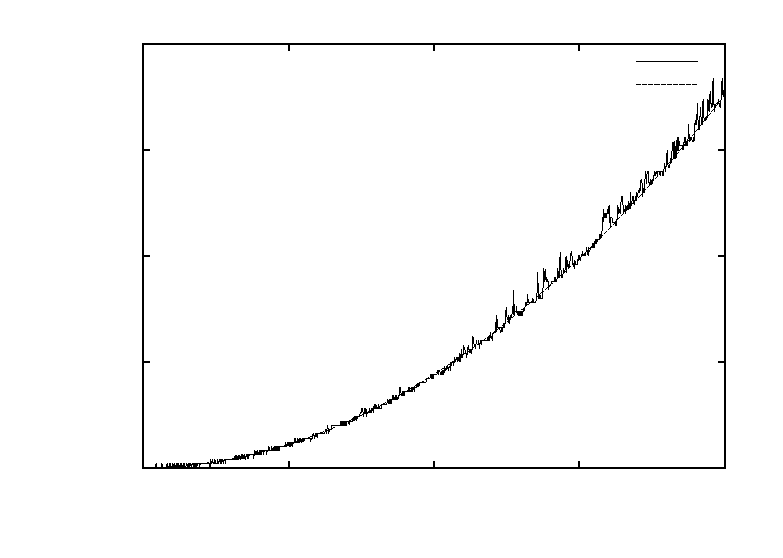
\includegraphics{insert_sort_timing.eps}}%
    \gplfronttext
  \end{picture}%
\endgroup

\caption{Run time for sort. The program was run 500 times for each
  value of $n$ and the $y$-axis gives the total run time in seconds on
  my laptop, while I was also doing other things like typing this
  document and playing music videos on youtube. The code for doing the
  timing test is \texttt{  insert\_sort\_timing.c}. The $n^2$ behavior is
  clearly visible and the curve $0.88(n/1000)^2$ is plotted too, this
  was fitted by eye but is so good a fit it is hard to see it behind
  the run time data.\label{fig_insert_sort_timing}}
\end{figure}

So, to summarise, we have looked at a sort algorithm, insert sort and
found an estimate of how the run times grows with $n$ for the worst
case. This is the most common way of analysing algorithms. This will
all be formalised in the next section. You might expect that
calculating the average, rather than worst, run time would be more
interesting. 

However, that's usually more difficult, it is often hard to think
about exactly what average means and it always involves making some
assumption about the distribution of the initial data. Furthermore, it
usually turns out that the average case usually has the same sort of
behavior as the worst case behavior. For example, for insert sort, you
might replace $i$ with $i/2$ in the sums to get the average behavior,
but that will still lead to $n^2$. We will look at a case, quick sort,
where the worst behavior is very unusual, so a measure of the
\lq{}general case\rq{} is more useful.

One thing to realise is that the leading order behavior dominates,
that in choosing an algorithm, if $n$ is large, and these issues
really only matter is $n$ is large, the leading order behavior,
$O(n^2)$ or $O(n)$ or whatever, is what's important, not the precise
coefficients. Once the algorithm is chosen, if speed is very
important, then the code can be optimised to reduce the coefficient of
the leading term. However, it is worth noting that it is the leading
term that dominated so any optimizations should be directed at it's
coefficients, any trickery you do to speed up code is unlikely to have
a speed up bigger than the extra factor of $n$ or $\log{n}$ or
whatever separating the leading and sub-leading terms. In other words,
in the example given here, it is only worth worrying about reducing
$t_{10}$, $t_{11}$ and $t_{12}$. This is sometimes summed up with the
slogan: \lq{}never optimize outside the inner loop\rq{}. In short, for
most of your code, keep it readable and easy to update, but for the
inner loop, if speed is important, squeeze out all the optimizations
you can.


\subsection*{Big Oh notation}

The \lq{}Big Oh\rq{} notation has already been used to describe the
behavior of the running time of insert sort, we said
\begin{equation}
T(n)\in O(n^2)
\end{equation}
Here we want to formalize this notation. Basically $O(n^2)$ is a set
of functions, it is all the functions which, for large values of $n$ go
to infinity like $n^2$ at the fastest. By saying $T(n)\in O(n^2)$ we
are saying that $T(n)$ is one of these functions, its large $n$
behavior is, at worst, like $n^2$. 

Specifically, the definition of $O(g(n))$, called \lq{}big oh\rq{} of
$g(n)$, is
\begin{equation}
O(g(n))=\{f(n)| \exists n_0>0\in \textbf{ N}\mbox{ and }c>0\in \textbf{ R}\mbox{ with }|f(n)|\le c|g(n)|\,\forall n\ge n_0\}
\end{equation}
This definition is quite dense, but we can break it down: it says that
$O(g(n))$ is a set of functions, the curly brackets mean
\lq{}set\rq{}. $f(n)$ is in the set if it has a particular
property: the \lq$|$\rq{} can be read as \lq{}such that\rq{} or
\lq{}with the property that\rq{} and so this is the set of $f(n)$'s
where $f(n)$ has the property on the right of the $|$. Now,
\lq{}$\exists$\rq{} means \lq{}there exists\rq{} and
\lq{}$\forall$\rq{} means \lq{}for all\rq{}, so the defining property
says it is possible to find a positive natural number $n_0$ and a
positive real number $c$ so that if you choose a value of $n$ at
least as big as $n_0$ then $f(n)$ is no bigger than $cg(n)$, $\textbf{ N}$
and $\textbf{ R}$ stand for the natural and real numbers. Notice the
absolute value signs, this is about $|f(n)|$ and $|g(n)|$, in fact,
here we are interested in run times, so we will deal with functions
that are non-negative, or are non-negative provided $n$ is larger than
some threshold, for example, $\log_2{n}$ will be important,
$\log_2{n}$ is positive provided $n>1$.

In short, $f(n)$ can do all sorts of crazy stuff for small values of
$n$ but, if you take $n$ large enough, its behavior is bounded by the
behavior of $g(n)$. Now it doesn't say it is bounded by $g(n)$, it is
a statement about the behavior, that's the role of the $c$.

Here are some examples, say 
\begin{equation}
T(n)=5n^2+n+6
\end{equation}
then 
\begin{equation}
T(n)\in O(n^2)
\end{equation}
This means that $T(n)$ gets big at the same rate as $n^2$. As far as the definition is concerned, it means that we can choose an $n_0$ and a $c$ so that
\begin{equation}
cn^2\ge 5n^2+n+6
\end{equation}
for all $n>n_0$; it is easy to see that this should be possible, as
long as the $c>5$ the $n+6$ won't matter as $n$ gets large. In fact,
by, for example, taking $c=5+1+6=12$ then
\begin{equation}
12n^2\ge 5n^2+n+6
\end{equation}
provided $n\ge 1$ so $n_0=1$ here. 

However, 
\begin{equation}
T(n)\not\in O(n)
\end{equation}
In other words, no matter what $c$ and $n_0$ we choose there will be an $n>n_0$ such that
\begin{equation}
cn<5n^2+n+6
\end{equation}
and, again, it is easy to see this might be the case. Say we chosen
some value $c$ then
\begin{equation}
5n^2+n+6>cn
\end{equation}
for large enough $n$, to check this divide both sides by $n$ so we need to show that $n$ can be chosen so that
\begin{equation}
5n+1+\frac{6}{n}>c
\end{equation}
Since 
\begin{equation}
5n+1+\frac{6}{n}>5n+1
\end{equation}
then, if $n>c/5$
\begin{equation}
5n+1+\frac{6}{n}>5\frac{c}{5}+1=c+1>c
\end{equation}
so, no matter what value of $c$ is chosen, making $n>5/n$ implies
\begin{equation}
5n^2+n+6>cn
\end{equation}
so $5n^2+n+6\not\in O(n)$. 

In practice, if
\begin{equation}
T(n)=a_rn^r+a_{r-1}n^{r-1}+\ldots+a_1n+a_0
\end{equation}
then $T(n)\in O(n^r)$. We will recap this and look at other functions in the next chapter.

\end{document}

